\documentclass[10pt,twocolumn,letterpaper]{article}

\usepackage{cvpr}
\usepackage{times}
\usepackage{epsfig}
\usepackage{graphicx}
\usepackage{amsmath}
\usepackage{amssymb}
\usepackage{mathtools}
\usepackage{multicol}

\DeclarePairedDelimiter\abs{\lvert}{\rvert}%

% Include other packages here, before hyperref.

% If you comment hyperref and then uncomment it, you should delete
% egpaper.aux before re-running latex.  (Or just hit 'q' on the first latex
% run, let it finish, and you should be clear).
\usepackage[breaklinks=true,bookmarks=false]{hyperref}

\cvprfinalcopy % *** Uncomment this line for the final submission

\def\cvprPaperID{****} % *** Enter the  Paper ID here
\def\httilde{\mbox{\tt\raisebox{-.5ex}{\symbol{126}}}}

% Pages are numbered in submission mode, and unnumbered in camera-ready
\setcounter{page}{1}
\begin{document}

%%%%%%%%% TITLE
\title{EE3-23: Coursework for Introduction to Machine Learning}

\author{Douglas Brion\\
Imperial College London\\
CID: 01052925\\
{\tt\small db1415@ic.ac.uk}
}

\maketitle
%\thispagestyle{empty}


%%%%%%%%% BODY TEXT
\section{Introduction}

This report examines different approaches to predicting wine quality using the Wine Quality~\cite{WineQuality} dataset. This is a large dataset containing 4898 samples of white wines and 1599 of red. Throughout this report wine quality is examined using regression, the standard approach when modelling continuous data, attempting to predict the quality of a wine from various input parameters. Multiple learning methods are implemented, discussed and compared in order to obtain a predictor with the smallest test error possible.

All code for this report was written in Python using the libraries Pandas~\cite{mckinneypandas} for importing and manipulating data and Tensorflow~\cite{tensorflow2015-whitepaper} for creating and training models to predict the data.

%-------------------------------------------------------------------------
\section{Data Preparation}
Ad red and white wine have different tastes, it was decided to learn on both separately as they have a different chemical composition. The white wine dataset contains 4898 samples and the red 1599. The objective in this report is to establish how well the quality of each wine can be predicted using the datasets.

It should be noted that this data is likely to be unreliable with a large amount of noise as quality is measured with a human sense, taste a very personal sense which can range widely person to person.

The data provided was not normalised, therefore each attribute was normalised with respect to it's mean and standard deviation. Outliers over a threshold of for each attribute were removed to reduce noise in the dataset for training. Table \ref{tab:normalisedw} and Table \ref{tab:normalisedr} show the normalised physiochemical attributes for the datasets with outliers removed. 

\begin{figure}[h]
	\begin{center}
		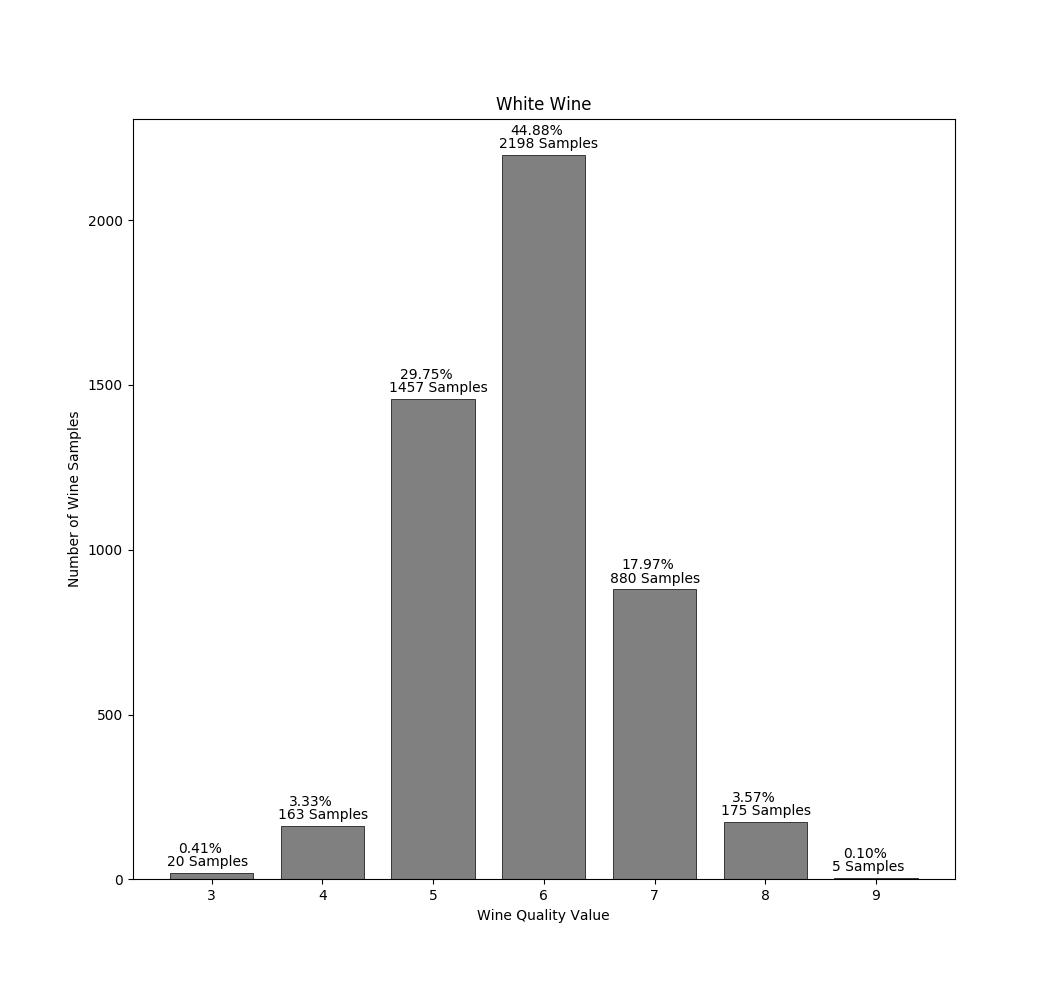
\includegraphics[width=0.9\linewidth]{img/white_samples.png}
	\end{center}
	\caption{The histogram for white wine qualities.}
	\label{fig:hist}
\end{figure}

\begin{figure}[h]
	\begin{center}
		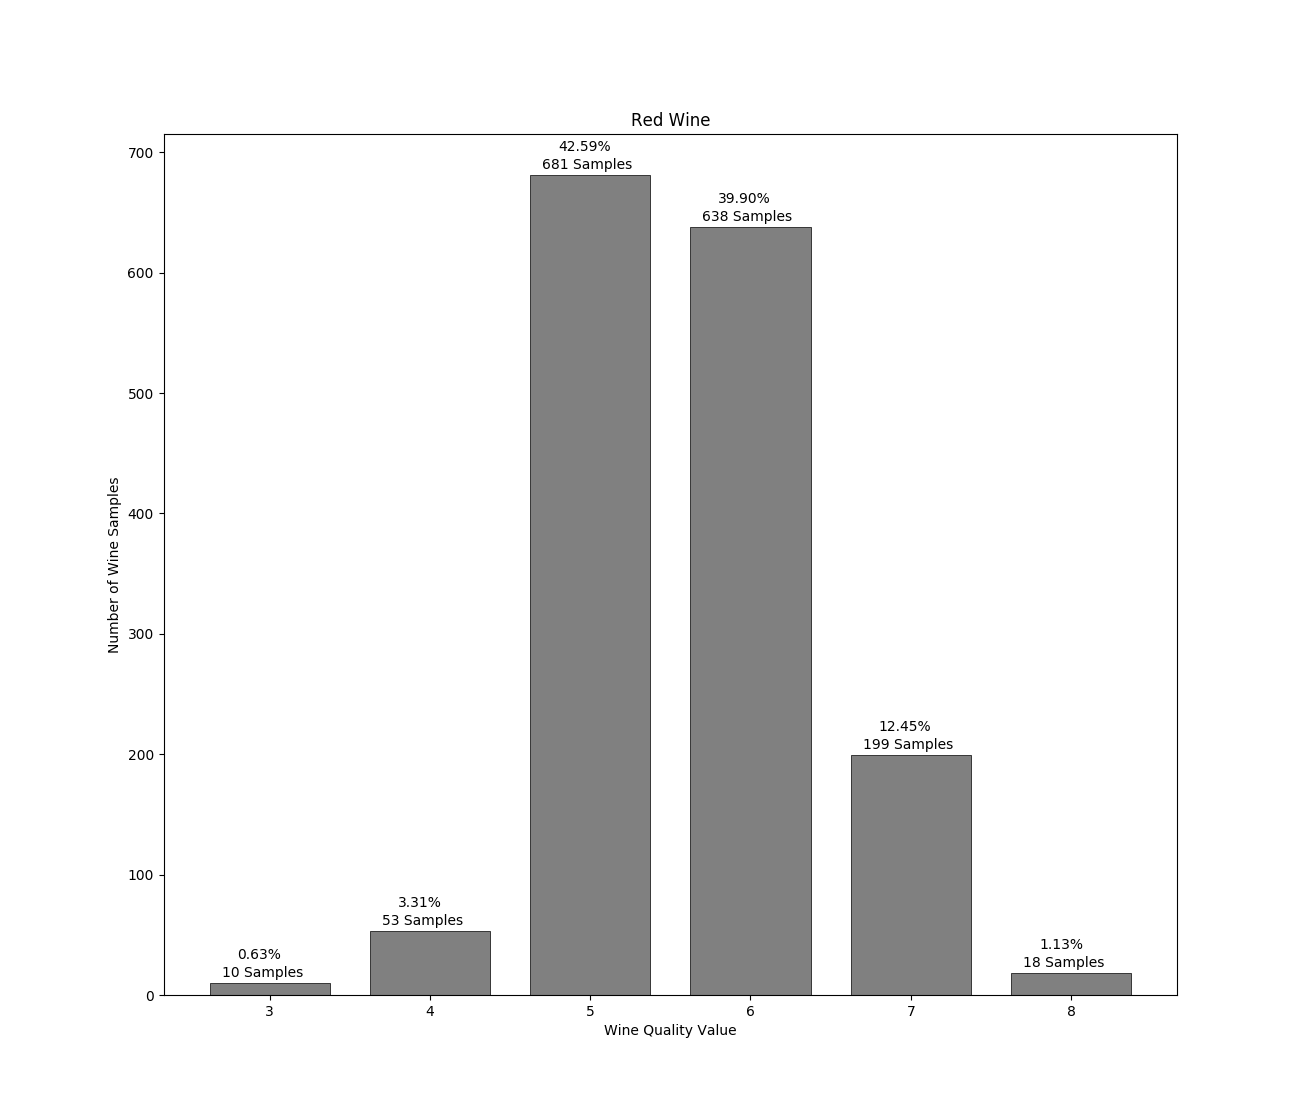
\includegraphics[width=0.9\linewidth]{img/red_samples.png}
	\end{center}
	\caption{The histogram for red wine qualities.}
	\label{fig:histr}
\end{figure}

\begin{table}[h]
	\begin{center}
		\begin{tabular}{|l|c|c|c|c|}
			\hline
			Attributes & Mean & Std & Min & Max \\
			\hline
			fixed acidity & -0.003 & 0.989 & -3.62 & 4.557 \\
			volatile acidity & -0.012 & 0.961 & -1.967 & 4.979 \\
			citric acid & -0.010 & 0.963 & -2.762 & 4.758 \\
			residual sugar & -0.002 & 0.986 & -1.142 & 4.971 \\
			chlorides & -0.078 & 0.662 & 1.683 & 4.954 \\
			free sulfur dioxide & -0.010 & 0.956 & -1.959 & 4.892 \\
			total sulfur dioxide & -0.003 & 0.992 & -3.044 & 4.839 \\
			density & -0.005 & 0.971 & -2.313 & 2.984 \\
			pH & 0.000 & 1.000 & 3.101 & 4.184 \\
			sulphates & -0.001 & 0.997 & -2.365 & 4.996 \\
			alcohol & 0.000 & 1.000 & -2.043 & 2.995 \\ 
			\hline
		\end{tabular}
	\end{center}
	\caption{The white wine attribute statistics after removal of outliers and normalisation.}
	\label{tab:normalisedw}
\end{table}

\begin{table}[h]
	\begin{center}
		\begin{tabular}{|l|c|c|c|c|}
			\hline
			Attributes & Mean & Std & Min & Max \\
			\hline
			fixed acidity & 0.000 & 1.000 & -2.137 & 4.355 \\
			volatile acidity & -0.004 & 0.989 & -2.278 & 4.481 \\
			citric acid & 0.000 & 1.000 & -1.391 &  3.744 \\
			residual sugar & -0.053 & 0.764 & -1.163 & 4.584 \\
			chlorides & -0.096 & 0.552 & -1.604 & 3.880 \\
			free sulfur dioxide & -0.003 & 0.991 & -1.423 & 4.985 \\
			total sulfur dioxide & -0.009 & 0.967 & -1.231 & 3.604 \\
			density & 0.000 & 1.000 & -3.539 & 3.680 \\
			pH & 0.000 & 1.000 & -3.700 & 4.528 \\
			sulphates & -0.033 & 0.879 & -1.936 & 4.142 \\
			alcohol & 0.000 & 1.000 & -1.899 & 4.202 \\ 
			\hline
		\end{tabular}
	\end{center}
	\caption{The red wine attribute statistics after removal of outliers and normalisation.}
	\label{tab:normalisedr}
\end{table}

The spread in quality for both data sets is not ideal with the histograms Fig \ref{fig:hist} and Fig \ref{fig:histr} illustrating the distribution. The quality of the wine is graded on a scale from 0 (really bad) to 10 (extremely good) with the datasets containing six/seven classes (3 to 8/9).

The goal of this project will be to find a predictor with the best regression performance.

\subsection{Learning approach}

For consistency all the different regressions performances of each model with varying parameters and training cost functions will be measured using the same error metric, the Huber Loss function. This is a good loss function for this regression problem as it is robust to outliers, for if the difference between the real and predicted value is small it will be squared, if large, the absolute value will be taken.

\begin{equation}
L_H = \begin{cases}
\sum_{i = 1}^{n} \frac{1}{2} (y_i - f(x_i))^2, & for \abs{y_i - f(x_i)} \leq \delta. \\
\sum_{i = 1}^{n} \delta \abs{y_i - f(x_i)} - \frac{1}{2} \delta^2, & otherwise.
\end{cases}
\label{eq:1}
\end{equation}

A robust procedure for estimation, \textit{k}-fold cross validation~\cite{CrossValidation}, where data is divided into \textit{k} parts and with one subset tested at a time and remaining data used for training. This methods results in all data being used for both training and testing, however requires a longer computation time.

\section{Baseline Predictors}
Several baseline predictors have been implemented and trained on the data. 

A linear regression program was written in Python using Tensorflow~\cite{tensorflow2015-whitepaper}. This linear model used an iterative method to alter the weights, with multiple loss functions tested. This proved useful as a framework for the more advanced algorithms implemented later on.

For linear regression 2 basic loss functions were implemented first.

\subsection{L1 loss function}
The $L_1$ loss function, least absolute deviations, tries to minimise the absolute difference between the predicted and real values. The sum of all the differences for all the samples can be described as follows:

\begin{equation}
L_1 = \sum_{i = 1}^{n} \abs{y_i - f(x_i)}
\end{equation}

This is a fairly robust loss function which is not that affected by outliers.

\begin{figure}[h]
	\begin{center}
		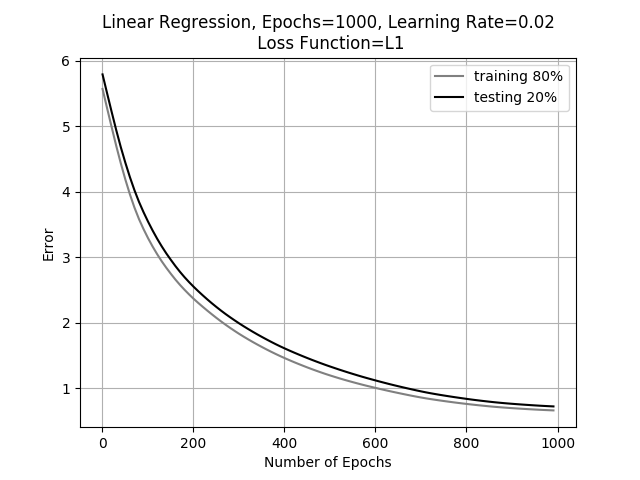
\includegraphics[width=0.9\linewidth]{img/l1loss.png}
	\end{center}
	\caption{Loss Function = $\sum_{i = 1}^{n} \abs{y_i - f(x_i)}$, Training Error = 0.321, Testing Error = 0.373}
	\label{fig:l1loss}
\end{figure}

\subsection{L2 loss function}
The $L_2$ loss function, least square error, minimises the square difference between the predicted and real values. This value is much large than that of $L_1$ loss and therefore is more affected by outliers, however, will optimise the predictor faster.

\begin{equation}
L_2 = \sum_{i = 1}^{n} (y_i - f(x_i))^2
\end{equation}

\begin{figure}[h]
	\begin{center}
		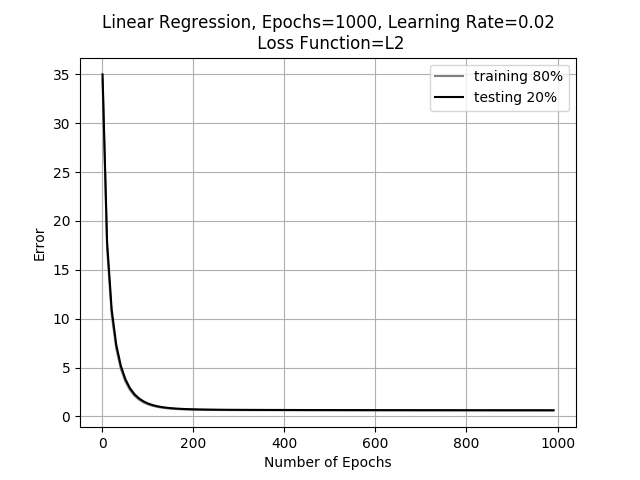
\includegraphics[width=0.9\linewidth]{img/l2loss.png}
	\end{center}
	\caption{Loss Function = $\sum_{i = 1}^{n} (y_i - f(x_i))^2$, Training Error = 0.271, Testing Error = 0.276}
	\label{fig:l2loss}
\end{figure}

Notice how the predictor using the $L_2$ loss function in \ref{fig:l2loss}. minimises the error much faster than the $L_1$ loss in \ref{fig:l1loss} and as outliers have been removed in data preparation the $L_2$ loss is quite robust.

As the epochs are increased the optimiser is able to reduce the loss until no improvements can be made. The learning rate also greatly affects the rate at which the loss is minimised. However, if the learning rate is too high the predictor will not improve on the training data, as can be seen in \ref{fig:break}.

\begin{figure}[h]
	\begin{center}
		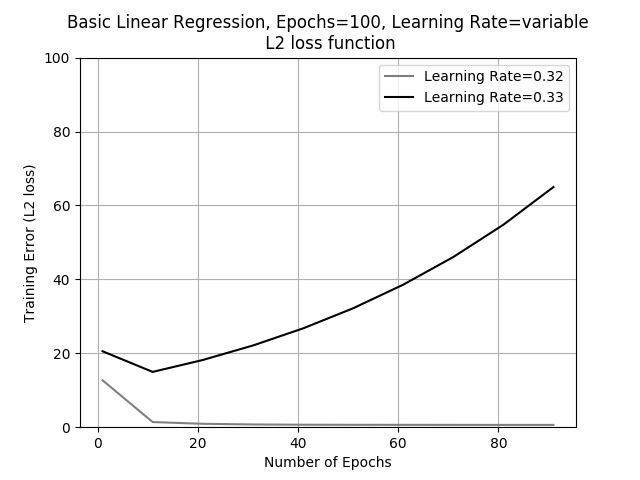
\includegraphics[width=0.9\linewidth]{img/linrbreak.png}
	\end{center}
	\caption{Training Error = $\sum_{i = 1}^{n} (y_i - f(x_i))^2$ ($L_2$ loss), Epochs = 100, Learning Rate = variable}
	\label{fig:break}
\end{figure}

\subsection{Improvements}
These relatively simple models can be improved upon by adding regularisation. Regularisation is a technique used to prevent over fitting the data. Both $L_1$ and $L_2$ regularisation have been implemented, being the sum of the weights and sum of the square weights respectively. The regularisation term is added to the loss function, the terms for $L_1$ and $L_2$ look as follows:

\noindent\begin{minipage}{.5\linewidth}
	\begin{equation}
	L_{1reg} = \lambda \sum_{i = 1}^{n} \abs{w_i}
	\end{equation}
\end{minipage}%
\begin{minipage}{.5\linewidth}
	\begin{equation}
	L_{2reg} = \lambda \sum_{i = 1}^{n} w_i^2
	\end{equation}
\end{minipage}

\section{More Advanced Algorithms}
More advanced algorithms such as NNs and SVMs achieve high performance due to their non-linear learning capabilities. However due to this, these complex models are more likely to over-fit, losing the ability to generalise when given new data to test. Both SVMs, NNs and Elastic Regularisation have multiple hyper-parameters which need to be adjusted in order to find the best predictor.

\subsection{Neural Network}
The neural network implemented as a predictor for this project had 3 layers, 1 input, 1 hidden and 1 output. A single hidden layer was chosen as an increase in hidden layers did not result in a significant increase in predictor performance although it did lengthen training time.

The number of nodes in the hidden was chosen using a heuristic of the number being the mean of the input and output layers, in this case resulting in 6 nodes.

Each layer could be assigned when the network is constructed to have a specific activation function such as: TanH, Sigmoid, ReLU, SeLU and Softmax. It was found that during training a hidden ReLU resulted in the best out of sample test error and therefore was chosen. 

Neural networks have an advantage over standard linear regression that they can model non-linearities automatically however they are more likely to over-fit the data so observing the out of sample error is especially important.

The neural net used a gradient descent optimiser to minimise the loss function, and either $L_1$, $L_2$ or no regularisation can be selected for training. 

\subsection{Support Vector Regression}
The goal for a support vector regression (SVR)~\cite{Cortes1995} predictor is to find a predication $f(x)$ like our other predictors however it should have at most $\epsilon$ deviation from the real value $y_i$ for all the in sample data.

The loss function for SVR is as follows:

\begin{equation}
L_{SVR} = max(0, \sum_{i = 1}^{n} \abs{y_i - f(x_i)} - \epsilon)
\end{equation}

This loss function is known as the hinge loss.

\subsection{Elastic Net Regularisation}
The elastic net regression is a regularised method combining the $L_1$ and $L_2$ penalties of the lasso and ridge methods. A hyper-parameter, $\alpha$ between 1 and 0 controls how much of $L_1$ and $L_2$ penalisation is used.

\section{Results}
In order to evaluate the possible models to find the best predictor, 10-fold cross validation was run for each model. Results graphs will illustrate the error of the model over the epochs with the final error for that models loss function shown as 'final error' in the legend. The final model after learning is then tested using Huber Loss \ref{eq:1} also shown in the legend. This is used to compare the various models against each other after training. The plots are the average cross validation errors of the predictor after each 10 epochs.

\subsection{Linear Regression}
For linear regression it was found that regularisation did not improve the performance of the predictor. As regularisation is used to help prevent over-fitting, and as basic linear regression is not as prone to over-fitting the data it was found that adding regularisation did not improve the performance.

\subsection{Neural Networks}
It was found that ReLU for both hidden and output layers was by far the most effective activation function. This may be because the ReLU function does not suffer from the vanishing gradient problem unlike functions such as tanh and sigmoid where the updating of weights can be prevented by a tiny gradient. 

It was also found that regularisation greatly improved the performance of neural net predictors. After running extensive tests with varying parameters and comparing the huber error of each of them, the best performing networks for both the white and red wine data sets can be seen below. Notice how Red wine has a smaller error as the quality is concentrated at values 5 and 6, this also may explain why $L_2$ regularisation fairs better.

Regularisation is especially important for the neural nets as they have a tendency to over-fit. However the regularisation parameter, $\lambda$ has to be tuned correctly to avoid not fitting the data at all.

Neural nets have a disadvantage over other methods proposed in this report as they may arrive a local minima during the learning phase, a problem algorithms such as SVRs do not encounter.

\begin{figure}[h]
	\begin{center}
		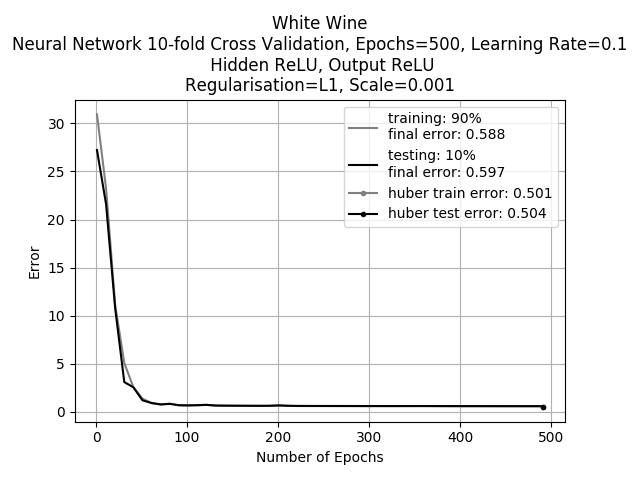
\includegraphics[width=0.9\linewidth]{img/best_white_nn.png}
	\end{center}
	\caption{Best Neural Network White Wine predictor.}
	\label{fig:wwbest}
\end{figure}

\begin{figure}[h]
	\begin{center}
		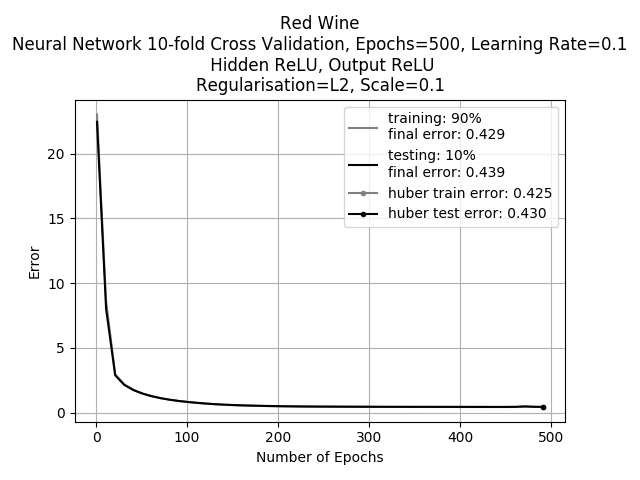
\includegraphics[width=0.9\linewidth]{img/best_red_nn.png}
	\end{center}
	\caption{Best Neural Network Red Wine predictor}
	\label{fig:rwbest}
\end{figure}

\subsection{Support Vector Regression}

\subsection{Elastic Net Regression}




{\small
\bibliographystyle{ieee}
\bibliography{egbib}
}

\end{document}
